\section{Campo com Autocomplete}

Nesta seção veremos como implementar um \texttt{autocomplete} para um
determinado campo de texto. Iremos transformar o campo \texttt{matricula} do
caso de uso \texttt{Consulta Estudante} em um campo com \texttt{autocomplete}.

O modelo inicial do caso de uso \texttt{Consulta Estudante} no  \texttt{CRUD}
para a entidade estudante pode ser visto na imagem \ref{modelo_consulta_estudante}:

\begin{figure}[H]
	\centering
	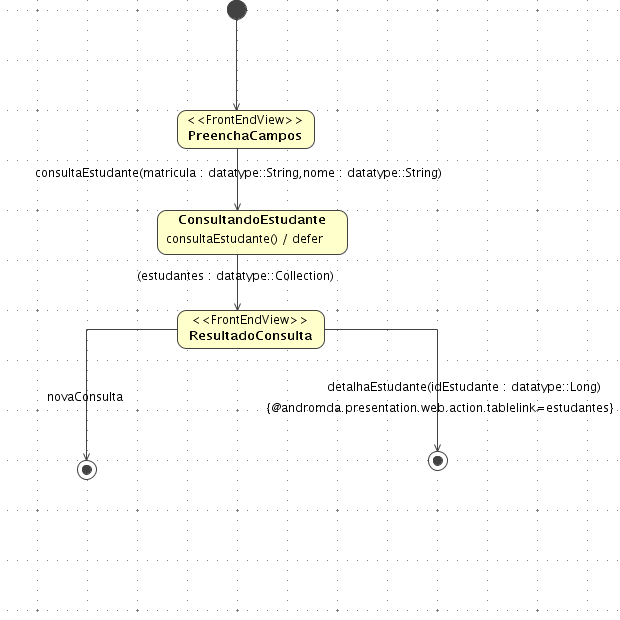
\includegraphics[width=350pt,height=300pt]{files/imgs/tutorial-mdarte-0028.png}
	\caption{Modelo do caso de uso Consulta Estudante.}
	\label{modelo_consulta_estudante}
\end{figure}

Abriremos a especificação da \texttt{transition} que sai da \texttt{front end
view} de nome \texttt{preencha os campos}, clicaremos no botão \texttt{edit}, no
\texttt{fieldset} \texttt{trigger}. Na aba \texttt{parameters}, da janela
\texttt{signal event specification}, que será aberta automaticamente, dê duplo
clique no nome do parâmetro \texttt{matricula} e será então aberta a
especificação do parâmetro. Selecione então a aba \texttt{tagged values},
selecione o \texttt{tagged value}
\texttt{@andromda.presentation.web.view.field.type} e clique no botão
\texttt{create value}. Selecione então a opção \texttt{autocomplete}, como na
imagem \ref{field_type_autocomplete}.

\begin{figure}[H]
	\centering
	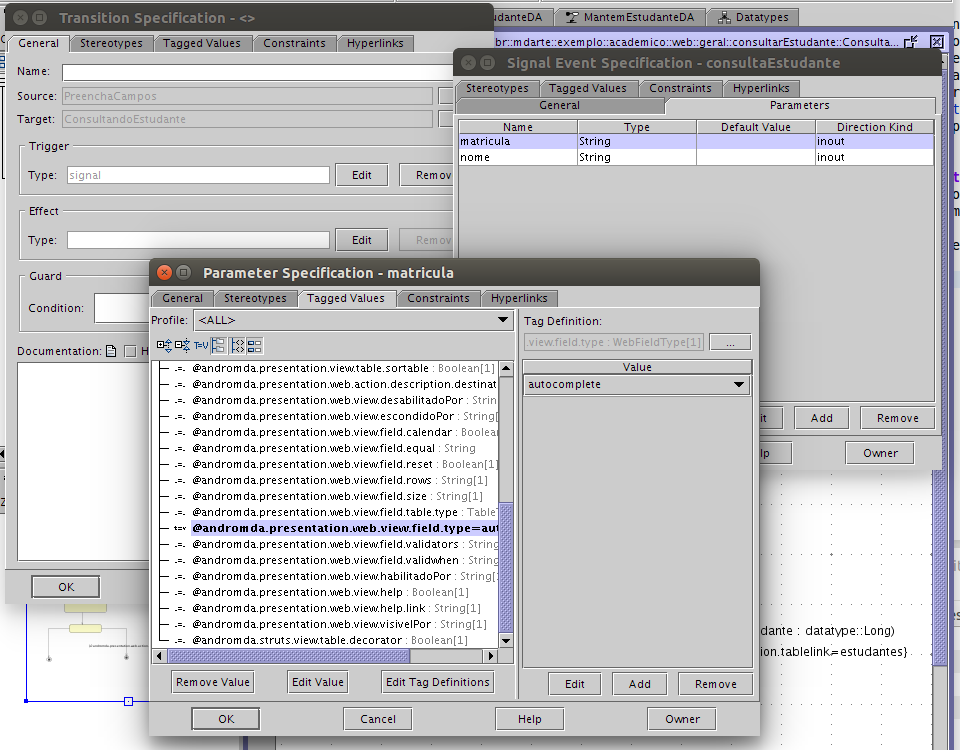
\includegraphics[width=350pt,height=300pt]{files/imgs/tutorial-mdarte-0027.png}
	\caption{Adicionando o field type 'autocomplete' à um campo da view.}
	\label{field_type_autocomplete}
\end{figure}

Agora executaremos o seguinte comando no terminal na raiz do projeto:
\begin{lstlisting}[language=bash]
maven mda -Dprojeto=sistemaacademico-geral-Estudante
\end{lstlisting}

Feito isto, o \texttt{MDArte} gerará automaticamente toda a estrutura
responsável por receber e tratar as requisições assíncronas para o preenchimento do
\texttt{autocomplete}, restando ao desenvolver apenas implementar no
\texttt{ControleImpl} a filtragem dos valores retornados, de acordo com o valor
do campo. Para isto, criaremos, na classe
\texttt{ConsultaEstudanteControleImpl}, um método seguindo o seguinte padrão 
\texttt{protected String[]
<nome-do-campo><nome-do-caso-de-uso>AutoComplete(java.lang.String query,
org.andromda.bpm4struts.ViewContainer container)}. Vejamos abaixo um exemplo de
implementação para o \texttt{autocomplete} do nosso campo de \texttt{matrícula}:

\lstinputlisting[language=java, frame=single, breaklines=true] {files/java/autocomplete.java}

Agora executaremos o seguinte comando para compilar e dar \texttt{deploy} no
\texttt{Sistema Acadêmico} :

\begin{lstlisting}[language=bash, frame=single, breaklines=true]
maven compile deploy
\end{lstlisting}

Feito isto, daremos \texttt{start} no \texttt{JBoss} e abriremos o sistema e
faremos login. Na tela \texttt{Preencha os Campos} do caso de uso
\texttt{Consulta Estudante} podemos agora verificar o \texttt{autocomplete}
funcionando, como na imagem \ref{exemplo_autocomplete}.

\begin{figure}[H]
	\centering
	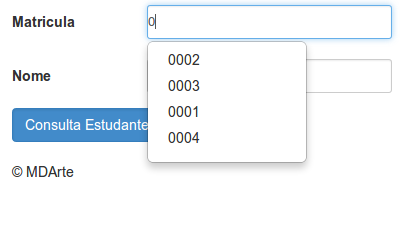
\includegraphics[width=350pt,height=300pt]{files/imgs/tutorial-mdarte-0029.png}
	\caption{Exemplo de autocomplete.}
	\label{exemplo_autocomplete}
\end{figure}